% Options for packages loaded elsewhere
\PassOptionsToPackage{unicode}{hyperref}
\PassOptionsToPackage{hyphens}{url}
%
\documentclass[
]{article}
\usepackage{amsmath,amssymb}
\usepackage{iftex}
\ifPDFTeX
  \usepackage[T1]{fontenc}
  \usepackage[utf8]{inputenc}
  \usepackage{textcomp} % provide euro and other symbols
\else % if luatex or xetex
  \usepackage{unicode-math} % this also loads fontspec
  \defaultfontfeatures{Scale=MatchLowercase}
  \defaultfontfeatures[\rmfamily]{Ligatures=TeX,Scale=1}
\fi
\usepackage{lmodern}
\ifPDFTeX\else
  % xetex/luatex font selection
\fi
% Use upquote if available, for straight quotes in verbatim environments
\IfFileExists{upquote.sty}{\usepackage{upquote}}{}
\IfFileExists{microtype.sty}{% use microtype if available
  \usepackage[]{microtype}
  \UseMicrotypeSet[protrusion]{basicmath} % disable protrusion for tt fonts
}{}
\makeatletter
\@ifundefined{KOMAClassName}{% if non-KOMA class
  \IfFileExists{parskip.sty}{%
    \usepackage{parskip}
  }{% else
    \setlength{\parindent}{0pt}
    \setlength{\parskip}{6pt plus 2pt minus 1pt}}
}{% if KOMA class
  \KOMAoptions{parskip=half}}
\makeatother
\usepackage{xcolor}
\usepackage[margin=1in]{geometry}
\usepackage{graphicx}
\makeatletter
\def\maxwidth{\ifdim\Gin@nat@width>\linewidth\linewidth\else\Gin@nat@width\fi}
\def\maxheight{\ifdim\Gin@nat@height>\textheight\textheight\else\Gin@nat@height\fi}
\makeatother
% Scale images if necessary, so that they will not overflow the page
% margins by default, and it is still possible to overwrite the defaults
% using explicit options in \includegraphics[width, height, ...]{}
\setkeys{Gin}{width=\maxwidth,height=\maxheight,keepaspectratio}
% Set default figure placement to htbp
\makeatletter
\def\fps@figure{htbp}
\makeatother
\setlength{\emergencystretch}{3em} % prevent overfull lines
\providecommand{\tightlist}{%
  \setlength{\itemsep}{0pt}\setlength{\parskip}{0pt}}
\setcounter{secnumdepth}{-\maxdimen} % remove section numbering
\ifLuaTeX
  \usepackage{selnolig}  % disable illegal ligatures
\fi
\IfFileExists{bookmark.sty}{\usepackage{bookmark}}{\usepackage{hyperref}}
\IfFileExists{xurl.sty}{\usepackage{xurl}}{} % add URL line breaks if available
\urlstyle{same}
\hypersetup{
  pdftitle={gloBarAnalysis},
  pdfauthor={ian enochs},
  hidelinks,
  pdfcreator={LaTeX via pandoc}}

\title{gloBarAnalysis}
\author{ian enochs}
\date{2024-03-10}

\begin{document}
\maketitle

\hypertarget{global-bmu-analysis}{%
\subsubsection{GLOBAL BMU Analysis}\label{global-bmu-analysis}}

This document was created to analyze NCRMP BMU data

\begin{verbatim}
## 
## Attaching package: 'dplyr'
\end{verbatim}

\begin{verbatim}
## The following objects are masked from 'package:stats':
## 
##     filter, lag
\end{verbatim}

\begin{verbatim}
## The following objects are masked from 'package:base':
## 
##     intersect, setdiff, setequal, union
\end{verbatim}

\begin{verbatim}
## 
## Attaching package: 'lubridate'
\end{verbatim}

\begin{verbatim}
## The following objects are masked from 'package:base':
## 
##     date, intersect, setdiff, union
\end{verbatim}

\hypertarget{qaqc-of-deltamass_mgcm2y}{%
\subsection{QA/QC of deltaMass\_mgcm2y}\label{qaqc-of-deltamass_mgcm2y}}

Tags where deltaMass\_mgcm2y = ``NA'':

\begin{verbatim}
## numeric(0)
\end{verbatim}

Historgram of deltaMass\_mgcm2y values
\includegraphics{gloBarAnalysis_files/figure-latex/unnamed-chunk-4-1.pdf}

\hypertarget{qaqc-of-deltavolume_mm3cm2y}{%
\subsection{QA/QC of
deltaVolume\_mm3cm2y}\label{qaqc-of-deltavolume_mm3cm2y}}

Tags where deltaVolume\_mm3cm2y = ``NA'':

\begin{verbatim}
##  [1] 2178 2181 2182 2183 2184 1321 1322 1323 1324 1325 4860 4861 4862 4863 4864
## [16] 4865 4866 4867 4869 4875 4877 4878 4870 4871 4872 4873 4881 4882 4883 4885
## [31] 4886 4887 4888 4889 4890 4891 4892 4893 4894 4896 4897 4898 4899 1027 3263
## [46] 3233 3229 4723
\end{verbatim}

Historgram of deltaVolume\_mm3cm2y values

\begin{verbatim}
## Warning: Removed 48 rows containing non-finite outside the scale range
## (`stat_bin()`).
\end{verbatim}

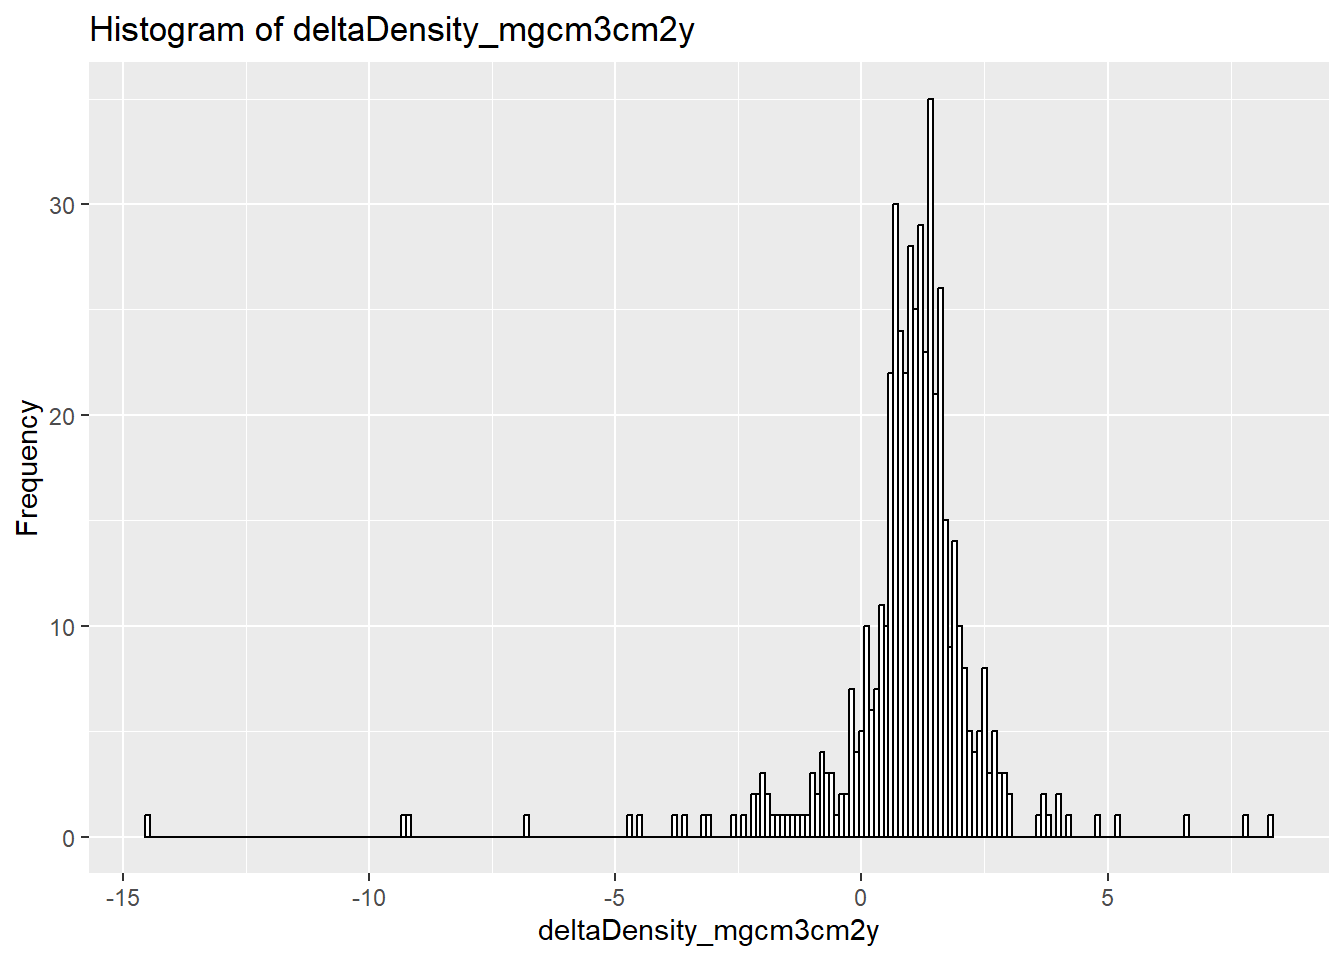
\includegraphics{gloBarAnalysis_files/figure-latex/unnamed-chunk-6-1.pdf}

\hypertarget{qaqc-of-deltadensity_mgcm3cm2y}{%
\subsection{QA/QC of
deltaDensity\_mgcm3cm2y}\label{qaqc-of-deltadensity_mgcm3cm2y}}

Tags where deltaDensity\_mgcm3cm2y = ``NA'':

\begin{verbatim}
##   [1] 4981 4982 4983 4984 4985 4980 1321 1322 1323 1324 1325 4860 4861 4862 4863
##  [16] 4864 4865 4866 4867 4869 4875 4877 4878 4870 4871 4872 4873 4881 4882 4883
##  [31] 4885 4886 4887 4888 4889 4890 4891 4892 4893 4894 4896 4897 4898 4899 1054
##  [46] 1058 1032 1033 1044 1051 1052 1055 1060 1034 1043 1046 1048 1053 1064 1065
##  [61] 1028 1030 1031 1035 1018 1021 1022 1023 1024 1025 1026 1027 1012 1013 1015
##  [76] 1016 1019 1001 1002 1009 1010 1011 1074 1076 1005 1079 1081 1003 1004 1082
##  [91] 1008 1045 1083 1084 1085 1086 1087 1089 1090 1096 3263 3233 1080 1088 1091
## [106] 1233 3229 1094 1097 1231 1066 1067 1068 1069 1078 1093 1099 1232 3245 3247
## [121] 4723
\end{verbatim}

Historgram of deltaDensity\_mgcm3cm2y values

\begin{verbatim}
## Warning: Removed 121 rows containing non-finite outside the scale range
## (`stat_bin()`).
\end{verbatim}

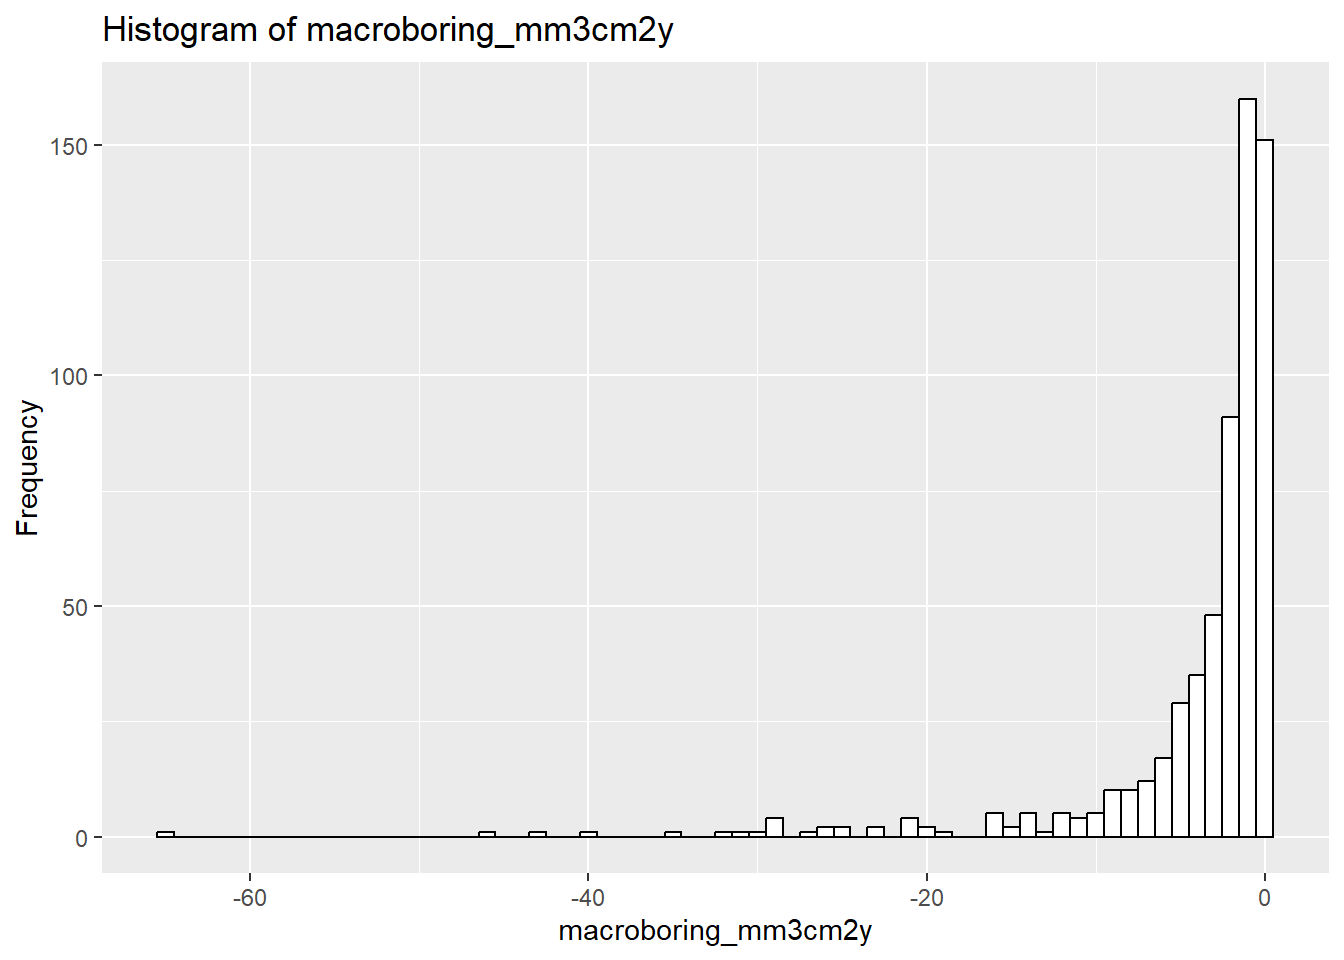
\includegraphics{gloBarAnalysis_files/figure-latex/unnamed-chunk-7-1.pdf}

\hypertarget{qaqc-of-macroboring_mm3cm2y}{%
\subsection{QA/QC of
macroboring\_mm3cm2y}\label{qaqc-of-macroboring_mm3cm2y}}

Tags where macroboring\_mm3cm2y = ``NA'':

\begin{verbatim}
## numeric(0)
\end{verbatim}

Historgram of macroboring\_mm3cm2y values
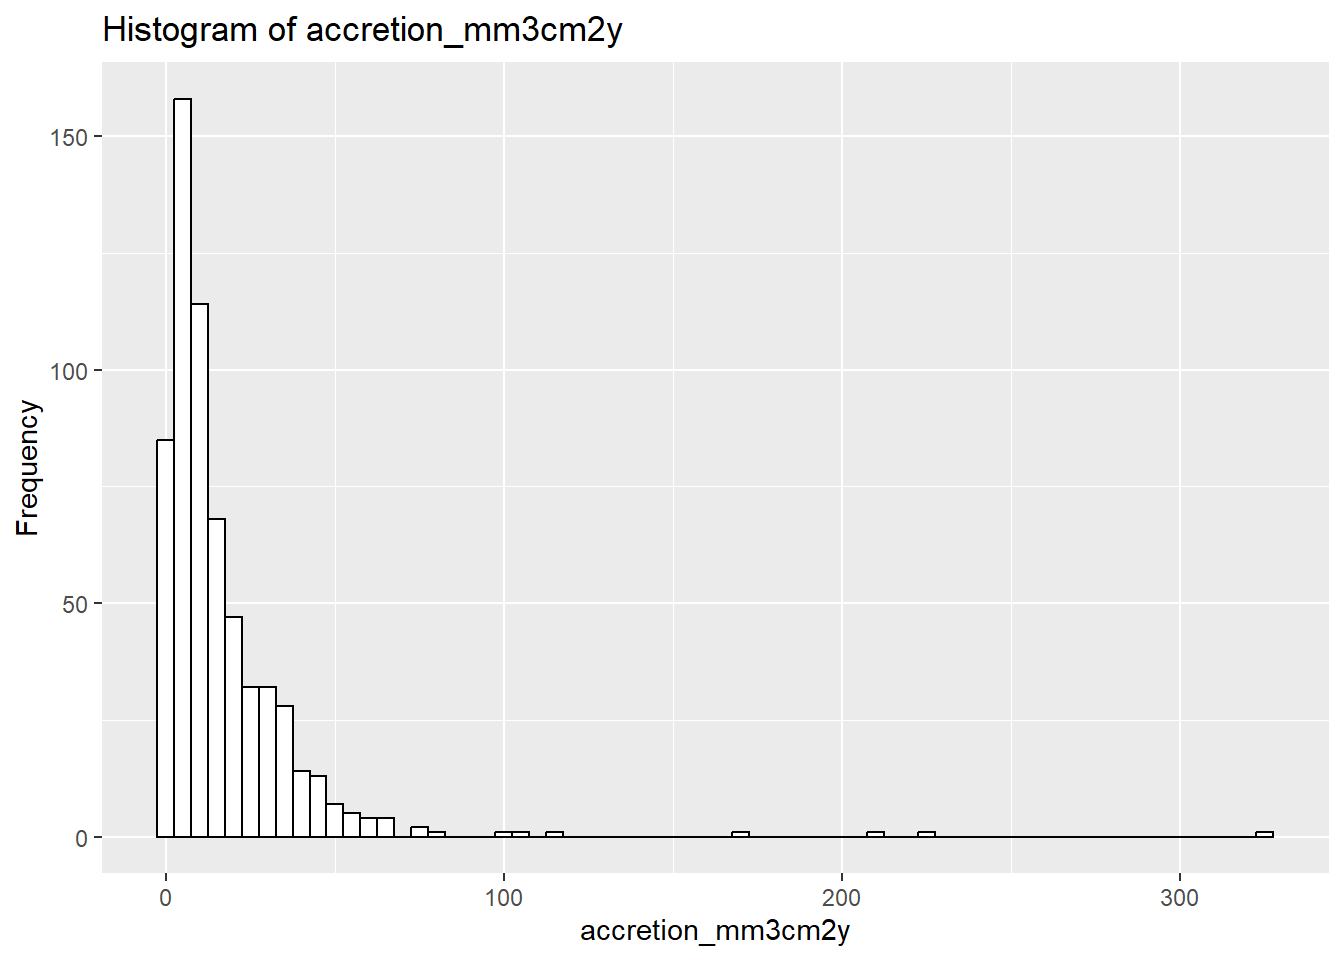
\includegraphics{gloBarAnalysis_files/figure-latex/unnamed-chunk-8-1.pdf}

\hypertarget{qaqc-of-accretion_mm3cm2y}{%
\subsection{QA/QC of
accretion\_mm3cm2y}\label{qaqc-of-accretion_mm3cm2y}}

Tags where accretion\_mm3cm2y = ``NA'':

\begin{verbatim}
## numeric(0)
\end{verbatim}

Historgram of accretion\_mm3cm2y values
\includegraphics{gloBarAnalysis_files/figure-latex/unnamed-chunk-9-1.pdf}

\hypertarget{qaqc-of-grazing_mm3cm2y}{%
\subsection{QA/QC of grazing\_mm3cm2y}\label{qaqc-of-grazing_mm3cm2y}}

Tags where grazing\_mm3cm2y = ``NA'':

\begin{verbatim}
##  [1] 2178 2181 2182 2183 2184 1321 1322 1323 1324 1325 4860 4861 4862 4863 4864
## [16] 4865 4866 4867 4869 4875 4877 4878 4870 4871 4872 4873 4881 4882 4883 4885
## [31] 4886 4887 4888 4889 4890 4891 4892 4893 4894 4896 4897 4898 4899 3263 3233
## [46] 3229 4723
\end{verbatim}

Historgram of grazing\_mm3cm2y values

\begin{verbatim}
## Warning: Removed 47 rows containing non-finite outside the scale range
## (`stat_bin()`).
\end{verbatim}

\includegraphics{gloBarAnalysis_files/figure-latex/unnamed-chunk-10-1.pdf}

\end{document}
